\documentclass[paper=a4,fontsize=11pt]{eucv}					
\begin{document}

\begin{minipage}{.2\linewidth}
   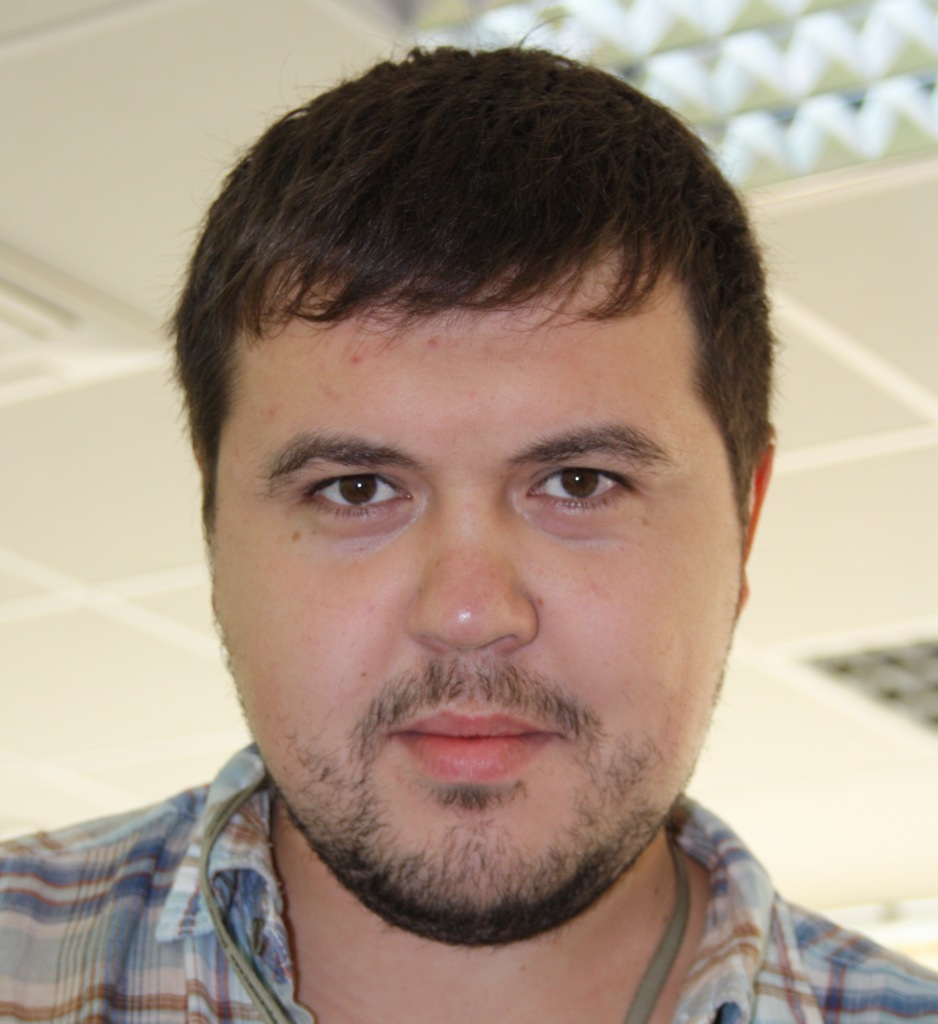
\includegraphics[width=1\textwidth]{userpic}
\end{minipage}      
\begin{minipage}{0.7\linewidth}
   \MyName{ Alexey Sibirtsev}
   \sepspace
   \noindent
   
   \hfill Berlin, Germany

   \hfill \MyEmail{alexey.sibirtsev@gmail.com}%
   
   \hfill \href{https://sibirtsev.com/}{sibirtsev.com}%
   
   \hfill +49 1525 876 64 43%
   
   \hfill \MySkype{alexey.sibirtsev}%
\end{minipage}


\NewPart{Skills}
\hspace{3mm}
\begin{minipage}[t]{0.33\textwidth} 
	
	\begin{tabular}[t]{ l l }
		\textbf{php} & 10+ years \\
		\textbf{nginx} & 10+ years \\
		\textbf{apache} & 10+ years \\
		\textbf{mysql} & 10+ years \\
		\textbf{mongodb} & 5+ years \\
		\textbf{python} & 1+ years \\
	\end{tabular}
	
	\sepspace
	
\end{minipage}
%
\begin{minipage}[t]{0.33\textwidth} 
	
	\begin{tabular}[t]{ l l }
		\textbf{html} & 10+ years \\
		\textbf{javascript} & 10+ years \\
		\textbf{css} & 2+ years \\
		\textbf{machine learning} & 1+ years \\
		\textbf{sphinxsearch} & 9+ years \\
		\textbf{symfony} (v2 - v6) & 5+ year
	\end{tabular}
	
	\sepspace
	
\end{minipage}
%
\begin{minipage}[t]{0.33\textwidth} 
	\begin{tabular}[t]{l l}
		memcache[d] & redis \\
		elasticsearch & aws \\
		linux & c++  \\
		git & bash \\
		agile & scrum  \\
		kanban & etc. \\
	\end{tabular}
\end{minipage}

\NewPart{Work experience}
\noindent

\WorkEntry{AUTO1 Group}{October 2020 - Now}{Team Lead Software Engineer }{
\noindent

    \textbf{Responsibilities}:
    \begin{itemize}
        \item Manage cross-functional team
        \item Design and development of backend part of application for internal usage
        \item Maintain existing products of the company
    \end{itemize}
    \sepspace

\noindent

    \textbf{Technologies}:
    \begin{itemize}
        \item Microservice architecture, RESTful API
        \item PHP 7, MySQL, Symfony Framework, Docker, PHPUnit, Behat
        \item AWS: S3, EC2, ECS, SQS, SNS, Lambda
    \end{itemize}
}
\sepspace

\WorkEntry{FlixMobility Tech GmbH}{June 2020 - Oktober 2020}{Senior Software Engineer }{
\noindent

    \textbf{Technologies}:
    \begin{itemize}
        \item PHP 7, MySQL, Postgres, Symfony Framework, Docker, PHPUnit, Behat, AWS
    \end{itemize}
}
\sepspace

\WorkEntry{AUTO1 Group}{May 2018 - May 2020}{Senior Software Engineer, Team Lead }{
\noindent

    \textbf{Responsibilities}:
    \begin{itemize}
        \item Design and development of backend part of internal application
        \item Maintain existing products of the company
        \item Manage cross-functional team
    \end{itemize}
    \sepspace

\noindent

    \textbf{Technologies}:
    \begin{itemize}
        \item Microservice architecture, RESTful API, GraphQL
        \item PHP, MySQL, Postgres, Symfony, Docker, PHPUnit, Behat
        \item AWS
    \end{itemize}
}
\sepspace

\pagebreak

\NewPart{Work experience \small{(continued)}}
\noindent
\WorkEntry{N1 Tech (NGS Tech, NGS)}{Jul 2007 - Apr 2018}{Head of Dev, Dev Lead, Data Scientist, Senior Developer }{
\noindent

	\textbf{Projects}:
	\begin{itemize}
		\item \textbf{realty.ngs.ru} -- property search site. Functions: project architecture development, programming, task management, team management
		\item \textbf{passport.ngs.ru} -- cross-domain authorization and access control service. Functions: project architecture development, programming, task management
		\item \textbf{n1.ru} -- property search site, new product. Functions: project architecture development, programming, task management, team management
	\end{itemize}

\sepspace
\noindent
	\textbf{Tasks}:
	\begin{itemize}
		\item Image classification with convolution neural network -- the classifier of the images of announcements on 7 classes: the facade of a building, a room, a kitchen, a bathroom, an entrance, a view from a window, the scheme of an apartment, based on caffe framework
		\item Real estate price tracking system -- the system for collecting and analyzing property price data, based on php and mysql
	\end{itemize}
}

\sepspace

\WorkEntry{eQuality Solutions}{May 2006 - Jul 2007 }{Lotus/Domino Developer}{%
Development and support of the company's products for foreign customers
}

\sepspace

\NewPart{Education}
\noindent

\EducationEntry{Specialist (Alumnus). Electronics and Microelectronics}{2009}{Novosibirsk State Technical University, Novosibirsk, Russia}{}

\sepspace

\NewPart{Social Links}
\noindent

\begin{tabular}[t]{ l l l l l }
	\href{https://www.linkedin.com/in/alexeysibirtsev/}{LinkedIn} & \href{https://www.facebook.com/alexey.sibirtsev}{Facebook} &  \href{https://github.com/Sibirtsev/}{GitHub} \\
\end{tabular}

\end{document}
